\subsection*{空间几何体的结构特征、表面积和体积}
\begin{enumerate}
    \item (2025$\cdot$杨浦区一模$\cdot$7)已知一个正四棱锥的每一条棱长都为 2，则该四棱锥的体积为\blkda[2]{$\dfrac{4\sqrt{2}}{3}$}.
    \begin{jieda}
        $V = \dfrac{1}{3} \times 4 \times \sqrt{2} = \dfrac{4\sqrt{2}}{3}$
    \end{jieda}

    \item (2025$\cdot$闵行区二模$\cdot$7)已知圆锥底面半径为 1，高为 $\sqrt{3}$ ，则过圆锥母线的截面面积的最大值为\blkda[2]{$\sqrt{3}$}.
    \begin{jieda}
        母线长为$2$，母线最大夹角为$\dfrac{\pi}{3}$，故轴截面为面积最大截面，$S = \dfrac{1}{2} \times 2 \times 2 \times \dfrac{\sqrt{3}}{2} = \sqrt{3}$.
    \end{jieda}

    \item (2024$\cdot$浦东新区一模$\cdot$7)已知圆锥的母线与底面所成的角为 $\dfrac{\pi }{3}$ ，体积为 ${3\pi }$ ，则圆锥的底面半径为\blkda[2]{$\sqrt{3}$}.
    \begin{jieda}
        $V = \dfrac{1}{3}\pi {r}^{2}h = \dfrac{1}{3}\pi {r}^{2} \times  \sqrt{3}r = {3\pi } \Longrightarrow  r = \sqrt{3}$.
    \end{jieda}

    \item (2024$\cdot$金山区一模$\cdot$7)已知某圆台上底面和下底面的半径分别为1 和 2， 母线长为 3，则该圆台的高为\blkda[2]{$2\sqrt{2}$}.
    \begin{jieda}
        作出圆台的轴截面, 如图示为等腰梯形, 梯形的高即为圆台的高, 即高为 $\sqrt{{3}^{2} - {\left( 2 - 1\right) }^{2}} = 2\sqrt{2}$.
        \begin{center}
            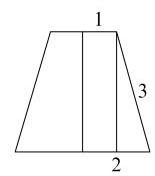
\includegraphics[width=0.15\textwidth]{bodyxb/src/107_664_274_155_176_0.jpg}
        \end{center}
    \end{jieda}

    \item (2025$\cdot$上海秋季卷$\cdot$7)如图所示，在正四棱柱 ${ABCD} - {A}_{1}{B}_{1}{C}_{1}{D}_{1}$ 中， ${BD} = 4\sqrt{2},{DB}_{1} = 9$ ，则该正四棱柱的体积为\blkda[2]{$112$}.
    \begin{center}
    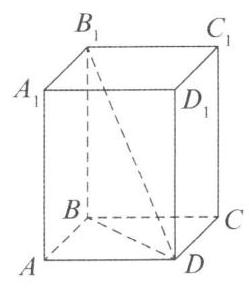
\includegraphics[width=0.2\textwidth]{bodyxb/src/144_1221_389_249_289_0.jpg}
    \end{center}
    \begin{jieda}
        因为 ${BD} = 4\sqrt{2}$ 且四边形 ${ABCD}$ 为正方形,故 ${BA} = 4$，而 $D{B}_{1} = 9$ ,故 $B{B}_{1}^{2} + B{D}^{2} = {81}$ ,故 $B{B}_{1} = 7$ ,故所求体积为 $7 \times  {16} = {112}$.
    \end{jieda}

    \item (2025$\cdot$宝山区二模$\cdot$8)已知圆柱的底面积为$9\pi$，侧面积为$18\pi$，则该圆柱的体积为\blkda[2]{${27\pi }$}.
    \begin{jieda}
        设圆柱的底面圆的半径为 $r$ ,高为 $h$，故有 $\left\{ \begin{array}{l} \pi {r}^{2} = {9\pi } \\  {2\pi rh} = {18\pi } \end{array}\right.$，解得 $\left\{ \begin{array}{l} r = 3 \\  h = 3 \end{array}\right.$，所以圆柱的体积$V = \pi {r}^{2}h = {27\pi }.$
    \end{jieda}

    \item (2025$\cdot$普陀区二模$\cdot$8)若一个圆锥的高为 $\sqrt{2}$ ，侧面积为 $2\sqrt{2}\pi$ ，则该圆锥侧面展开图中扇形的中心角的大小为\blkda[2]{$\sqrt{2}\pi$}.
    \begin{jieda}
        设底面半径为 $r$ ,母线长为 $l$ ,由 ${\pi rl} = 2\sqrt{2}\pi$ ,得 ${rl} =  2\sqrt{2}$ ,又 $h = \sqrt{2}$ ,由勾股定理 $l = \sqrt{{r}^{2} + 2}$ ,所以 $r\sqrt{{r}^{2} + 2} =  2\sqrt{2}$ ,解得 $r = \sqrt{2},l = 2$ ,底面圆周长 $L = {2\pi r} = 2\sqrt{2}\pi$ ,扇形中心角 $\theta  = \dfrac{L}{l} = \dfrac{2\sqrt{2}\pi }{2} = \sqrt{2}\pi$.
    \end{jieda}

    \item (2024$\cdot$普陀区一模$\cdot$8)设圆锥的底面中心为 $O$ ， ${PB}$ 、 ${PC}$ 是它的两条母线，且 $\left| {BC}\right|  = 2$ ，若棱锥 $O - {PBC}$ 是正三棱锥，则该圆锥的侧面积为\blkda[2]{$2\sqrt{2}\pi$}.
    \begin{jieda}
        由棱锥 $O - {PBC}$ 为正三棱锥，得 ${PB} = {PC} = {BC} = 2,{OB} = {OC} =  {OP}$ ,而 ${PO} \bot  {OB},{PO} \bot  {OC}$ ,由勾股定理得 ${OB} = {OC} = {OP} = \sqrt{2}$ ,即圆锥的底面圆半径 $r = \sqrt{2}$ ,母线长 $l = 2$ ,则该圆锥的侧面积为 ${\pi rl} = 2\sqrt{2}\pi$.
        \begin{center}
        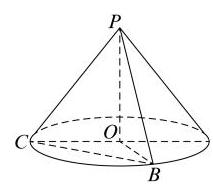
\includegraphics[width=0.2\textwidth]{bodyxb/src/107_605_1091_213_191_0.jpg}
        \end{center}
    \end{jieda}

    \item (2025$\cdot$普陀区一模$\cdot$8)若圆锥 $P - O$ 的体积为 $\dfrac{2\sqrt{2}\pi }{3}$ ，它的母线与底面所成的角的余弦值为 $\dfrac{1}{3}$ ， 则圆锥 $P - O$ 的表面积为\blkda[2]{${4\pi }$}.
    \begin{jieda}
        设圆锥底面半径 ${AO} = {OB} = r$ ,则母线长 $l = {PA} =  {3r}$ ,高 ${PO} = 2\sqrt{2}r$ ,则 $V = \dfrac{1}{3}\pi {r}^{2} \cdot  2\sqrt{2}r = \dfrac{2\sqrt{2}}{3}\pi$ ,解得 $r = 1$ , $l = {PA} = 3,{PO} = 2\sqrt{2}$ ,故该圆锥的表面积为 $S = {\pi rl} + \pi {r}^{2} =  {4\pi }$.
    \end{jieda}

    \item (2025$\cdot$青浦区一模$\cdot$8)已知圆柱 $M$ 的底面半径为3，高为 $\sqrt{3}$ ，圆锥 $N$ 的底面直径和母线长相等. 若圆柱 $M$ 和圆锥 $N$ 的体积相同，则圆锥 $N$ 的底面半径为\blkda[2]{3}.
    \begin{jieda}
        圆柱 $M$ 的体积为 $\pi  \cdot  {3}^{2} \times  \sqrt{3} = 9\sqrt{3}\pi$ ,设圆锥 $N$ 的底面半径为 $r$ ,则母线长为 ${2r}$ ,故圆锥的高为 $\sqrt{{\left( 2r\right) }^{2} - {r}^{2}} =  \sqrt{3}r$ ,则 $\dfrac{1}{3}\pi  \cdot  {r}^{2} \cdot  \sqrt{3}r = \dfrac{\sqrt{3}}{3}\pi {r}^{3}$ ,故 $\dfrac{\sqrt{3}}{3}\pi {r}^{3} = 9\sqrt{3}\pi$ ,解得 $r = 3$.
    \end{jieda}

    \item (2025$\cdot$奉贤区二模$\cdot$8)抛物线 ${x}^{2} = {4y}$ 的准线与圆 ${x}^{2} + {y}^{2} = {r}^{2}$ 相切，将圆绕直径所在直线旋转一周形成一个几何体，则该几何体的表面积为\blkda[2]{${4\pi }$}.
    \begin{jieda}
        因为抛物线方程为 ${x}^{2} = {4y}$ ,可知准线方程为 $y =$ -1,又由圆 ${x}^{2} + {y}^{2} = {r}^{2}$ 与准线相切,可知: $r = 1$ ,将圆绕直径旋转一周所成的球的表面积为: $S = {4\pi }$.
    \end{jieda}
\end{enumerate}
\subsection*{直线、平面平行的判定与性质}
\begin{enumerate}
    \item (2024$\cdot$静安区二模$\cdot$14)设$m$、$n$是两条不同的直线，$\alpha, \beta$是两个不同的平面，下列命题中真命题是 \dotfill{(\kh{C})}
    \xx{若 $m//\alpha ,n//\alpha$ ,则 $m//n$}{若 $m \subset  \alpha ,n \subset  \beta ,m//n$ ,则 $\alpha //\beta$}{若 $m \bot  \alpha ,n//\alpha$ ,则 $m \bot  n$}{若 $m \subset  \alpha ,n \subset  \alpha ,m//\beta ,n//\beta$ ,则 $\alpha //\beta$}

    \item (2024$\cdot$长宁区二模$\cdot$14)已知直线 $a$ 、 $b$ 和平面 $\alpha$ ，则下列判断中正确的是 \dotfill{(\kh{C})}
    \xx{若 $a//\alpha ,b//\alpha$，则 $a//b$}{若 $a//b,b//\alpha$，则 $a//\alpha$}{若 $a//\alpha ,b \bot  \alpha$，则 $a \bot b$}{若 $a \bot  b,b//\alpha$，则 $a \bot  \alpha$}

    \item (2023$\cdot$上海春季卷$\cdot$15)如图所示， $P$ 是正方体 ${ABCD} - {A}_{1}{B}_{1}{C}_{1}{D}_{1}$ 边 ${A}_{1}{C}_{1}$ 上的动点，下列哪条边与 ${BP}$ 边始终异面 \dotfill{(\kh{B})}
    \begin{center}
    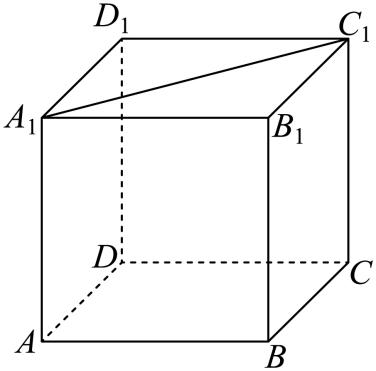
\includegraphics[width=0.2\textwidth]{bodyxb/src/152_1139_688_294_456_0.jpg}
    \end{center}
    \xx{$D{D}_{1}$}{${AC}$}{$A{D}_{1}$}{${B}_{1}C$}

    \item (2025$\cdot$浦东新区一模$\cdot$14)设$m$、$n$是两条不同的直线，$\alpha, \beta$是两个不同的平面，且 $\alpha \cap \beta = n$. 下述四个命题中为假命题的是 \dotfill{(\kh{B})}
    \xx{若 $m \bot  \alpha$ ，则 $m \bot  n$}{若 $m//\alpha$ ，则 $m//n$}{若 $m//\alpha$ 且 $m//\beta$ ，则 $m//n$}{若 $m//n$ ，则 $m//\alpha$ 或 $m//\beta$}

    \item (2024$\cdot$宝山区二模$\cdot$15)已知直线 $l$ 、 $m$ 、 $n$ 与平面 $\alpha$ 、 $\beta$ ，则下列命题中正确的是 \dotfill{(\kh{C})}
    \xx{若 $\alpha //\beta ,l \subset  \alpha ,n \subset  \beta$ ,则 $l//n$}{若 $\alpha  \bot  \beta ,l \subset  \alpha$ ,则 $l \bot  \beta$}{若 $l \bot  \alpha ,l//\beta$ ，则 $\alpha  \bot  \beta$}{若 $l \bot  n,m \bot  n$ ,则 $l//m$} 

    \item (2024$\cdot$青浦区一模$\cdot$15)已知直线 $m$ 、 $n$ ，平面 $\alpha$ 、 $\beta$. 给出下列命题:
    
    \ding{172}  若 $m\bot \alpha ,n\bot \beta$ ，且 $m\bot n$ ，则 $\alpha \bot \beta$ ；  \ding{173}  若 $m//\alpha ,n//\beta$ ，且 $m//n$ ，则 $\alpha //\beta$ ；

    \ding{174}  若 $m\bot \alpha ,n//\beta$ ，且 $m\bot n$ ，则 $\alpha \bot \beta$ ；  \ding{175}  若 $m\bot \alpha ,n//\beta$ ，且 $m//n$ ，则 $\alpha //\beta$.

    其中正确的命题的个数是 \dotfill{(\kh{A})}

    \xx{1}{2}{3}{4}
    \begin{jieda}
        对于 \ding{172} ,由 $m\bot \alpha$ ,且 $m\bot n$ ,得 $n//\alpha$ 或 $n \subset  \alpha$ ,又 $n\bot  \beta$ ,则 $\alpha  \bot  \beta$ , \ding{172} 正确
        
        对于 \ding{173} ,若 $m//\alpha ,n//\beta$ ,且 $m//n$ ,则 $\alpha$ 与 $\beta$ 平行或相交, \ding{173}  错误; 
        
        对于 \ding{174} ,若 $m \bot  \alpha ,n//\beta$ ,且 $m \bot  n$ ,则 $\alpha$ 与 $\beta$ 平行、垂直或斜交, \ding{174} 错误; 
        
        对于 \ding{175} ,由 $n//\beta$ ,得存在过直线 $n$ 的平面 $\gamma$ ,使得 $\beta  \cap  \gamma  = l$ ,则 $n//l$ ,而 $m//n$ ,则 $m//l$ ,又 $m \bot  \alpha$ ,则 $l \bot  \alpha$ ,又 $l \subset  \beta$ ,因此 $\alpha  \bot  \beta$ , \ding{175} 错误
    \end{jieda}


    \item (2024$\cdot$金山区一模$\cdot$15)如图，在正方体 ${ABCD} - {A}_{1}{B}_{1}{C}_{1}{D}_{1}$ 中， $E$ 、 $F$ 为正方体内 (含边界) 不重合的两个动点,下列结论错误的是 \dotfill{(\kh{D})}
    \begin{center}
    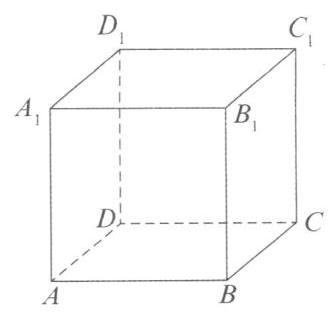
\includegraphics[width=0.2\textwidth]{bodyxb/src/152_1072_1681_335_315_0.jpg}
    \end{center}
    \xx{若 $E \in  B{D}_{1},F \in  {BD}$ ,则 ${EF} \bot  {AC}$}{若 $E \in  B{D}_{1},F \in  {BD}$ ,则平面 ${BEF} \bot$ 平面 ${A}_{1}B{C}_{1}$}{若 $E \in  {AC},F \in  C{D}_{1}$ ,则 ${EF}//$ 平面 ${A}_{1}B{C}_{1}$}{若 $E \in  {AC},F \in  C{D}_{1}$ ,则 ${EF}//A{D}_{1}$}
\end{enumerate}
\subsection*{直线、平面垂直的判定与性质}
\begin{enumerate}
    \item (2025$\cdot$长宁区一模$\cdot$14)已知非零空间向量 $\vv{a}$ 、 $\vv{b}$ 和 $\vv{c}$ ，则下列说法正确的是 \dotfill{(\kh{D})}
    \xx{若 $\vv{a}\bot \vv{b},\vv{a}\bot \vv{c}$ ,则 $\vv{b}//\vv{c}$}{若 $\vv{a}\bot \vv{b},\vv{a}\bot \vv{c}$ ,则 $\vv{b}\bot \vv{c}$}{若 $\vv{a}\bot \vv{b},\vv{a}//\vv{c}$ ,则 $\vv{b}//\vv{c}$}{若 $\vv{a}\bot \vv{b},\vv{a}//\vv{c}$ ,则 $\vv{b}\bot \vv{c}$}

    \item (2025$\cdot$嘉定区二模$\cdot$14)已知平面 $\alpha$ 和平面 $\beta$ ，直线 $m \subset  \alpha$ ，直线 $n \subset  \beta$ ，则下列结论一定成立的是 \dotfill{(\kh{D})}
    \xx{若 $m//n$ ，则 $\alpha //\beta$}{若 $m$ 与 $n$ 为异面直线，则 $\alpha //\beta$}{若 $m \bot  n$ ，则 $\alpha  \bot  \beta$}{若 $n \bot  \alpha$ ，则 $m \bot  n$}

    \item (2024$\cdot$上海春季卷$\cdot$14)空间中有两个不同的平面 $\alpha$ 、 $\beta$ ，两条不同的直线 $m$ 、 $n$ ，则下列说法正确的是 \dotfill{(\kh{A})}
    \xx{若 $\alpha  \bot  \beta ,m \bot  \alpha ,n \bot  \beta$ ,则 $m \bot  n$}{若 $\alpha  \bot  \beta ,m \bot  \alpha ,m \bot  n$ ,则 $n \bot  \beta$}{若 $\alpha //\beta ,m//\alpha ,n//\beta$ ,则 $m//n$}{若 $\alpha //\beta ,m//\alpha ,m//n$ ,则 $n//\beta$}

    \item (2025$\cdot$崇明区一模$\cdot$14)已知直线 $l$ 和平面 $\alpha$ ，则“$l$ 垂直于 $\alpha$ 内的两条直线”是“$l\bot \alpha$ ”的\dotfill{(\kh{B})}
    \xx{充分非必要条件}{必要非充分条件}{充要条件}{非充分非必要条件}

    \item (2025$\cdot$嘉定区一模$\cdot$14)已知 $\alpha$ 、 $\beta$ 是两个不同的平面， $a$ 、 $b$ 是两条不同的直线，下列条件中，一定得到直线 $l \bot  \alpha$ 的是 \dotfill{(\kh{C})}
    \xx{$\alpha  \bot  \beta ,l//\beta$}{$l \bot  a,a// \alpha$}{$l//a,a \bot  \alpha$}{$l \bot  a,l \bot  b,a \subset  \alpha ,b \subset  \alpha$}

    \item (2024$\cdot$奉贤区一模$\cdot$13)已知两个不同的平面 $\alpha$ 和 $\beta$ ， $m$ 为平面 $\alpha$ 内的一条直线，则“$\alpha \bot \beta$”是“$m \bot \beta$ ”的 \dotfill{(\kh{B})}
    \xx{充分非必要条件}{必要非充分条件}{充要条件}{既非充分也非必要条件}

    \item (2024$\cdot$金山区二模$\cdot$15)如图，点 $N$ 为正方形 ${ABCD}$ 的中心， $\bigtriangleup  {ECD}$ 为正三角形，平面 ${ECD}\bot$ 平面 ${ABCD},M$ 是线段 ${ED}$ 的中点,则以下命题中正确的是 \dotfill{(\kh{D})}
    \begin{center}
    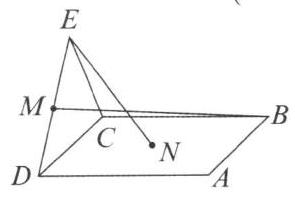
\includegraphics[width=0.2\textwidth]{bodyxb/src/156_1134_457_295_197_0.jpg}
    \end{center}
    
    \xx{${BM} = {EN}$}{${CD} \bot  {MN}$}{$A,M,N$ 三点共线}{直线 ${BM}$ 与 ${EN}$ 相交}
\end{enumerate}

\subsection*{空间向量}
\begin{enumerate}
    \item (2025$\cdot$徐汇区一模$\cdot$4)已知向量 $\vv{a} = \left( {2,5,1}\right) ,\vv{b} = \left( {4,m,5}\right)$ ，若 $\vv{a} \cdot  \vv{b} = 3$ ，则实数 $m$ 的值为\blkda[2]{$-2$}.

    \item (2024$\cdot$长宁区一模$\cdot$9)若向量 $\vv{a} = \left( {1,0,2}\right) ,\vv{b} = \left( {0,1, - 1}\right)$ ，则 $\vv{a}$ 在 $\vv{b}$ 方向上的投影向量的坐标为\blkda[2]{$\left( {0, - 1,1}\right)$}.
\begin{jieda}
    $\vv{a} \cdot  \vv{b} =  - 2$ , $\left| \vv{b}\right|  = \sqrt{2}$ ,所以 $\vv{a}$ 在 $\vv{b}$ 方向上的投影向量为 $\dfrac{\vv{a} \cdot  \vv{b}}{\left| \vv{b}\right| } \cdot  \dfrac{\vv{b}}{\left| \vv{b}\right| } =  - \vv{b} = \left( {0, - 1,1}\right)$.
\end{jieda}

    \item (2025$\cdot$浦东新区二模$\cdot$11)已知 $\vv{a}$ 、 $\vv{b}$ 、 $\vv{c}$ 为空间中三个单位向量，且 $\vv{a} \cdot  \vv{b} = \vv{b} \cdot  \vv{c} = \vv{c} \cdot  \vv{a} = 0$ ，若向量 $\vv{p}$ 满足 $\left| {\vv{p} - 2\vv{a}}\right|  = \dfrac{3}{2},\left| {\vv{p} - 2\vv{b}}\right|  = \dfrac{3}{2}$ ，则向量 $\vv{p}$ 与向量 $\vv{c}$ 夹角的最小值为\blkda[2]{$\arccos \dfrac{\sqrt{2}}{4}$}. (用反三角表示)
    \begin{jieda}
        可设 $\vv{a} = \left( {1,0,0}\right) ,\vv{b} = \left( {0,1,0}\right) ,\vv{c} = \left( {0,0,1}\right)$ ,设 $\vv{p} =  \left( {x,y,z}\right)$ ,则 $\vv{p} - 2\vv{a} = \left( {x - 2,y,z}\right) ,\vv{p} - 2\vv{b} = \left( {x,y - 2,z}\right)$ , 所以 $\left\{  \begin{array}{l} {\left( x - 2\right) }^{2} + {y}^{2} + {z}^{2} = \dfrac{9}{4} \\  {x}^{2} + {\left( y - 2\right) }^{2} + {z}^{2} = \dfrac{9}{4} \end{array}\right.$ ,两式相减可得: $x = y$ ,再代入第一个式子,可得: $2{x}^{2} + {z}^{2} = {4x} - \dfrac{7}{4}$ ,设向量 $\vv{p}$ 与向量 $\vv{c}$ 夹角为 $\theta$ ,则 $\cos \theta  = \dfrac{z}{\sqrt{{x}^{2} + {y}^{2} + {z}^{2}}} = \dfrac{\sqrt{{4x} - \dfrac{7}{4} - 2{x}^{2}}}{\sqrt{{4x} - \dfrac{7}{4}}} =  \sqrt{1 - \dfrac{2{x}^{2}}{{4x} - \dfrac{7}{4}}} = \sqrt{1 - \dfrac{2}{\dfrac{4}{x} - \dfrac{7}{4{x}^{2}}}}$ ,易知对于 $y =  - \dfrac{7}{4{x}^{2}} + \dfrac{4}{x}$ 当 $\dfrac{1}{x} = \dfrac{8}{7}$ 即 $x = \dfrac{7}{8}$ 取得最大值 $\dfrac{16}{7}$ ,此时 $\sqrt{1 - \dfrac{2}{\dfrac{4}{x} - \dfrac{7}{4{x}^{2}}}}$ 取得最大值 $\dfrac{\sqrt{2}}{4}$ ，即 $\cos \theta$ 的最大值为 $\dfrac{\sqrt{2}}{4}$ ， $x = \dfrac{7}{8}$ 时取得，再由余弦函数的单调性可知 $\theta$ 的最小值为 $\arccos \dfrac{\sqrt{2}}{4}$.
    \end{jieda}
    \item (2025$\cdot$普陀区二模$\cdot$11)在棱长为 4 的正方体 ${ABCD} - {A}_{1}{B}_{1}{C}_{1}{D}_{1}$ 中， $\vv{AN} = 2\vv{AM} = \dfrac{1}{2}\vv{A{C}_{1}}$ ，若一动点 $G$ 满足 $\left| \vv{GN}\right|  = \sqrt{2}\left| \vv{GM}\right|$ ，则三棱锥 $G - {A}_{1}{B}_{1}{D}_{1}$ 体积的最大值为\blkda[2]{$\dfrac{{32} + 8\sqrt{6}}{3}$}.
    \begin{jieda}
        如图,以 $A$ 为坐标原点建立空间直角坐标系,则有 $A\left( {0,0,0}\right) ,{C}_{1}\left( {4,4,4}\right)$ . 又 $\vv{AN} = 2\vv{AM} = \dfrac{1}{2}\vv{A{C}_{1}}$ ,所以 $M(1,1,1),N\left( {2,2,2}\right)$.
        
        设 $G\left( {x,y,z}\right)$ ,则 $\vv{GN} = (2 - x,2 - y,2 -  z),\vv{GM} = \left( {1 - x,1 - y,1 - z}\right)$ . 因为 $\left| \vv{GN}\right|  = \sqrt{2}\left| \vv{GM}\right|$ ,代入可得 ${\left( 2 - x\right) }^{2} + {\left( 2 - y\right) }^{2} + {\left( 2 - z\right) }^{2} = 2\left\lbrack {\left( 1 - x\right) }^{2} + {\left( 1 - y\right) }^{2} +{\left( 1 - z\right) }^{2}\right\rbrack$ ,整理可得 ${x}^{2} + {y}^{2} + {z}^{2} = 6$ ,即 $G$ 在以点 $A$ 为球心， $r = \sqrt{6}$ 为半径的球上. 又 ${{Rt}}\bigtriangleup {A}_{1}{B}_{1}{D}_{1}$ 的面积为 ${S}_{\bigtriangleup {A}_{1}{B}_{1}{D}_{1}} = \dfrac{1}{2} \times  4 \times  4 = 8$ ，平面 ${ABCD}$ 到平面 ${A}_{1}{B}_{1}{C}_{1}{D}_{1}$ 的距离为 4,所以 $G$ 到平面 ${A}_{1}{B}_{1}{D}_{1}$ 的最大距离为 ${d}_{\max } = 4 + r = 4 + \sqrt{6}$ . 体积最大值为 $V = \dfrac{1}{3} \times  {S}_{\bigtriangleup {A}_{1}{B}_{1}{D}_{1}} \times  {d}_{\max } = \dfrac{1}{3} \times  8 \times  \left( {4 + \sqrt{6}}\right)  = \dfrac{{32} + 8\sqrt{6}}{3}.$
        \begin{center}
        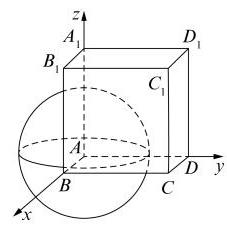
\includegraphics[width=0.2\textwidth]{bodyxb/src/111_1301_1944_227_225_0.jpg}
        \end{center}
    \end{jieda}
    \item (2025$\cdot$奉贤区二模$\cdot$14)如图所示，在平行六面体 ${ABCD} - {A}_{1}{B}_{1}{C}_{1}{D}_{1}$ 中，点 $N$ 在对角线 ${A}_{1}C$ 上，点 $M$ 在对角线 ${A}_{1}B$ 上， $\vv{{A}_{1}N} = \dfrac{1}{3}\vv{NC}$ ， $\vv{{A}_{1}M} = \dfrac{1}{2}\vv{MB}$ ，以下命题正确的是 \dotfill{(\kh{B})}
    \xx{$\vv{MN}//\vv{BC}$}{${D}_{1},N,M$ 三点共线}{${D}_{1}M$ 与 ${A}_{1}C$ 是异面直线}{$\vv{{D}_{1}N} = \dfrac{1}{2}\vv{NM}$}
    \begin{center}
    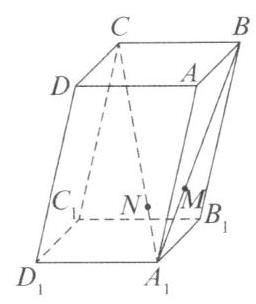
\includegraphics[width=0.15\textwidth]{bodyxb/src/151_1177_1042_256_304_0.jpg}
    \end{center}
    \begin{jieda}
        在平行六面体 ${ABCD} - {A}_{1}{B}_{1}{C}_{1}{D}_{1}$ 中,令 $\vv{AB} = \vv{a}$ , $\vv{AD} = \vv{b},\vv{A{A}_{1}} = \vv{c}$ ,则 $\vv{{A}_{1}B} = \vv{{A}_{1}A} + \vv{AB} =  - \vv{c} + \vv{a} = \vv{a} - \vv{c}$ , $\vv{{A}_{1}C} = \vv{{A}_{1}A} + \vv{AB} + \vv{BC} =  - \vv{c} + \vv{a} + \vv{b} = \vv{a} + \vv{b} - \vv{c}$
        
        $\vv{MN} =  \vv{M{A}_{1}} + \vv{{A}_{1}N} =  - \dfrac{1}{3}\vv{{A}_{1}B} + \dfrac{1}{4}\vv{{A}_{1}C} =  - \dfrac{1}{3}\left( {\vv{a} - \vv{c}}\right)  + \dfrac{1}{4}(\vv{a} +  \vv{b} - \vv{c}) =  - \dfrac{1}{12}\vv{a} + \dfrac{1}{4}\vv{b} + \dfrac{1}{12}\vv{c},\vv{BC} = \vv{AD} = \vv{b}$ ，因为 $\vv{a},\vv{b},\vv{c}$ 不共线，所以 $\vv{MN}$ 与 $\vv{BC}$ 不平行，故 A 错误；
        
        $\vv{{D}_{1}N} = \vv{{D}_{1}{A}_{1}} +  \vv{{A}_{1}N} =  - \vv{AD} + \dfrac{1}{4}\vv{{A}_{1}C} =  - \vv{b} + \dfrac{1}{4}\left( {\vv{a} + \vv{b} - \vv{c}}\right)  = \dfrac{1}{4}\vv{a} - \dfrac{3}{4}\vv{b} -  \dfrac{1}{4}\vv{c},\vv{MN} =  - \dfrac{1}{3}\vv{{D}_{1}N}$ ,即有 $\vv{MN}//\vv{{D}_{1}N},\vv{MN},\vv{{D}_{1}N}$ 有公共点 $N$ ，所以 ${D}_{1}$ 、 $N$ 、 $M$ 三点共线，B 选项正确；
        
        因为点 $N$ 在直线 ${D}_{1}M$ 上，点 $N$ 也在直线 ${A}_{1}C$ 上，所以 ${D}_{1}M$ 与 ${A}_{1}C$ 是相交直线,故 ${C}$ 选项错误
        
        因为 $\vv{MN} =  - \dfrac{1}{3}\vv{{D}_{1}N}$ ,所以 $\vv{{D}_{1}N} =  3\vv{NM}$ ，故 D 选项错误.
    \end{jieda}

    \item (2025$\cdot$黄浦区二模$\cdot$14)如图所示，在平行六面体 ${ABCD} - {A}_{1}{B}_{1}{C}_{1}{D}_{1}$ 中，设 $\vv{a} = \vv{A{A}_{1}},\vv{b} = \vv{D{B}_{1}}$ ，若 $\vv{a}$ 、 $\vv{b}$ 、 $\vv{c}$ 组成空间向量的一个基底，则 $\vv{c}$ 可以是\dotfill{(\kh{B})}
    \xx{$\vv{B{B}_{1}}$}{$\vv{B{C}_{1}}$}{$\vv{BD}$}{$\vv{B{D}_{1}}$}

    \begin{center}
    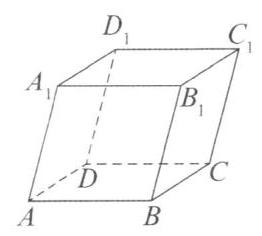
\includegraphics[width=0.15\textwidth]{bodyxb/src/151_1173_1408_262_236_0.jpg}
    \end{center}

    \item (2025$\cdot$虹口区一模$\cdot$15)已知边长为 2 的正四面体 $A - {BCD}$ 的内切球 (球面与四面体四个面都相切的球) 的球心为 $O$ ，若空间中的动点 $P$ 满足 $\vv{OP} = x\vv{OC} + y\vv{OB} + z\vv{OD},x,y,z \in  \left\lbrack  {0,1}\right\rbrack$ ,则点 $P$ 的轨迹所形成的几何体的体积为 \dotfill{(\kh{A})}

    \xx{$\sqrt{2}$}{$\dfrac{\sqrt{2}}{3}$}{$2\sqrt{3}$}{$\dfrac{\sqrt{3}}{3}$} 
    \begin{jieda}
        因为 $\vv{OP} = x\vv{OC} + y\vv{OB} + z\vv{OD},x,y,z \in  \left\lbrack  {0,1}\right\rbrack$ ,所以点 $P$ 的轨迹是以 ${OB},{OC},{OD}$ 为棱的平行六面体. 正四面体边长为 2,高 $h = \sqrt{{2}^{2} - {\left( \dfrac{2\sqrt{3}}{3}\right) }^{2}} = \sqrt{\dfrac{8}{3}} = \dfrac{2\sqrt{6}}{3}$ ,设正四面体 $A - {BCD}$ 的内切球半径为 $r$ ,则 $4 \times  \dfrac{1}{3} \times  \dfrac{\sqrt{3}}{4} \times  {2}^{2} \times  r =  \dfrac{1}{3} \times  \dfrac{\sqrt{3}}{4} \times  {2}^{2} \times  \dfrac{2\sqrt{6}}{3} \Longrightarrow  r = \dfrac{\sqrt{6}}{6}$ ,体积为 $V = 6{V}_{O - {BCD}} = 6 \times  \dfrac{1}{3} \times  \dfrac{\sqrt{3}}{4} \times  {2}^{2} \times  \dfrac{\sqrt{6}}{6} = \sqrt{2}$
        \begin{center}
        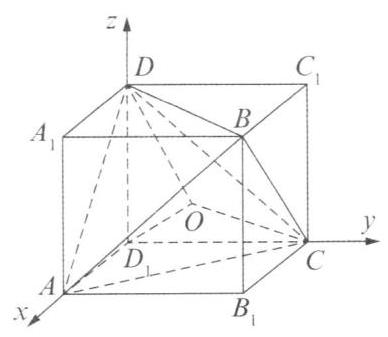
\includegraphics[width=0.2\textwidth]{bodyxb/src/151_1047_1698_388_337_0.jpg}
        \end{center}
    \end{jieda}
\end{enumerate}

\subsection*{空间角与距离}
\begin{enumerate}
    \item (2024$\cdot$杨浦区二模$\cdot$7)正方体 ${ABCD} = {A}_{1}{B}_{1}{C}_{1}{D}_{1}$ 中，异面直线 ${AB}$ 与 $D{C}_{1}$ 所成角的大小为\blkda[2]{$\dfrac{\pi }{4}$}.
    \begin{jieda}
        如图所示异面直线 ${AB}$ 与 $D{C}_{1}$ 所成角的大小为 $\angle {B}_{1}{AB} = \dfrac{\pi }{4}$.
        \begin{center}
    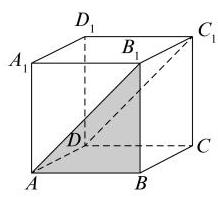
\includegraphics[width=0.2\textwidth]{bodyxb/src/117_598_1292_218_197_0.jpg}
    \end{center}
    \end{jieda}

    \item (2024$\cdot$崇明区一模$\cdot$7)在空间直角坐标系中，点 $P\left( {1, -2, 3}\right)$ 到 ${xOy}$ 平面的距离为\blkda[2]{3}.
    \begin{jieda}
        点 $P\left( {1, - 2,3}\right)$ 到 ${xOy}$ 平面的距离为 $d = \left| z\right|  = 3$.
    \end{jieda}

    \item (2025$\cdot$上海春季卷$\cdot$9)已知 $P$ 是一个圆锥的顶点， ${PA}$ 是母线， ${PA} = 2$， 圆锥的底面半径是 $1.B,C$ 分别在圆锥的底面上，则异面直线 ${PA}$ 与 ${BC}$ 所成角的最小值为\blkda[2]{$\dfrac{\pi }{3}$}.
    \begin{center}
    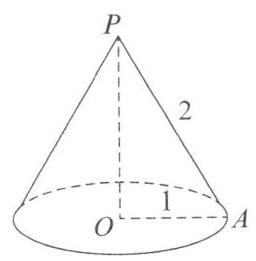
\includegraphics[width=0.2\textwidth]{bodyxb/src/159_1132_527_256_261_0.jpg}
    \end{center}
    \begin{jieda}
        线面角最小角定理: 直线 ${PA}$ 与底面上所有直线的夹角中,最小的角是 ${PA}$ 与底面的夹角,即 $\angle {PAO} = \dfrac{\pi }{3}$.
    \end{jieda}
    \item (2025$\cdot$金山区一模$\cdot$7)已知某圆锥的侧面展开图是圆心角为 $\sqrt{2}\pi$ 、半径为 2 的扇形，则该圆锥的母线与底面所成角的大小为\blkda[2]{$\dfrac{\pi }{4}$}.
    \begin{jieda}
        令底面半径为 $r$ ,则 ${2\pi r} = 2\sqrt{2}\pi$ ,可得 $r = \sqrt{2}$ ,且圆锥母线为 2 , 所以该圆锥的母线与底面所成角的余弦值为 $\dfrac{\sqrt{2}}{2}$ ,故其大小为 $\dfrac{\pi }{4}$.
    \end{jieda}

    \item (2024$\cdot$奉贤区一模$\cdot$5)在四面体 $P - {ABC}$ 中，若底面 ${ABC}$ 的一个法向量为 $\vv{n} = \left( {1,1,0}\right)$ ，且 $\vv{CP} = \left( {2,2, -1}\right)$ ，则顶点 $P$ 到底面 ${ABC}$ 的距离为\blkda[2]{$2\sqrt{2}$}.
    \begin{jieda}
        $d = \dfrac{\left| \vv{CP} \cdot  \vv{n}\right| }{\left| \vv{n}\right| } = \dfrac{1 \times  2 + 1 \times  2 + 0}{\sqrt{2}} = 2\sqrt{2}$.
    \end{jieda}

    \item (2024$\cdot$崇明区二模$\cdot$8)已知底面半径为 1 的圆柱， $O$ 是其上底面圆心， $A$ 、 $B$ 是下底面圆周上两个不同的点， ${BC}$ 是母线. 若直线 ${OA}$ 与 ${BC}$ 所成角的大小为 $\dfrac{\pi }{3}$ ，则 ${BC} =$ \blkda[2]{$\dfrac{\sqrt{3}}{3}$}.
    \begin{jieda}
        过点 $A$ 作与 ${BC}$ 平行的母线 ${AD}$ ,连接 ${OD}$ ,则 $\angle {OAD}$ 即为直线 ${OA}$ 与 ${BC}$ 所成的角,在 $\operatorname{Rt}\bigtriangleup {ODA}$ 中, $\tan \angle {OAD} = \dfrac{OD}{AD} = \dfrac{1}{AD} = \tan \dfrac{\pi }{3} = \sqrt{3}$ ，故 ${AD} = {BC} = \dfrac{\sqrt{3}}{3}$.
            \begin{center}
            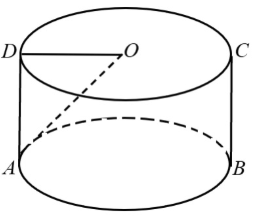
\includegraphics[width=0.2\textwidth]{bodyxb/src/24chongmingermo8.png}
            \end{center}
    \end{jieda}

    \item (2025$\cdot$崇明区一模$\cdot$9)在空间直角坐标系中，点(1，2，3)关于 ${xOy}$ 平面的对称点的坐标是\blkda[2]{$\left( {1,2, - 3}\right)$}.

    \item (2025$\cdot$徐汇区二模$\cdot$7)已知 ${PA}\bot$ 平面 ${ABC},{\bigtriangleup {ABC}}$ 是直角三角形，且 ${AB} = {AC} = 2,{PA} = 4$ ，则点 $P$ 到直线 ${BC}$ 的距离是\blkda[2]{$3\sqrt{2}$}.
    \begin{jieda}
        取 ${BC}$ 中点为 $D$ ,连接 ${AD}$ 、 ${PD}$ ,如图所示,因为 ${ABC}$ 为等腰三角形,又 $D$ 为 ${BC}$ 中点,故 ${BC} \bot  {AD}$ ; 因为 ${PA} \bot$ 平面 ${ABC},{BC} \subset$ 面 ${ABC}$ ,故 ${BC} \bot  {PA}$ ,又 ${AD},{PA} \subset$ 面 ${PAD},{AD} \cap  {PA} = A$ ,故 ${BC} \bot$ 平面 ${PAD}$ ,又 ${PD} \subset$ 平面 ${PAD}$ ,故 ${PD} \bot  {BC}$ ,故点 $P$ 到直线 ${BC}$ 的距离,即为 ${PD}$ ; 在 $\bigtriangleup {ABC}$ 中, ${AD} = \dfrac{1}{2}{BC} = \dfrac{1}{2} \times  \sqrt{2}{AB} = \sqrt{2}$ ; 因为 ${PA} \bot$ 平面 ${ABC},{AD} \subset$ 平面 ${ABC}$ ,故 ${PA} \bot  {AD}$ ,则 $\bigtriangleup {PAD}$ 为直角三角形; 在 $\bigtriangleup {PAD}$ 中, ${PA} = 4,{AD} = \sqrt{2}$ ,故 ${PD} =  \sqrt{P{A}^{2} + A{D}^{2}} = \sqrt{{16} + 2} = 3\sqrt{2}$ ,故点 $P$ 到直线 ${BC}$ 的距离为 $3\sqrt{2}$.

        \begin{center}
        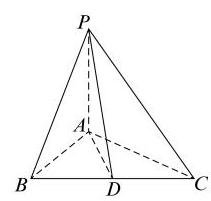
\includegraphics[width=0.2\textwidth]{bodyxb/src/117_1317_1197_211_201_0.jpg}
        \end{center}
    \end{jieda}

    \item (2025$\cdot$虹口区一模$\cdot$9)如图所示，已知正三角形 ${ABC}$ 和正方形 ${BCDE}$ 的边长均为 2，且二面角 $A - {BC} - D$ 的大小为 $\dfrac{\pi }{6}$ ，则 $\vv{AC} \cdot  \vv{BD} =$ \blkda[2]{$-1$}.
    \begin{center}
        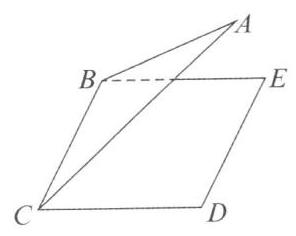
\includegraphics[width=0.2\textwidth]{bodyxb/src/159_619_1771_296_236_0.jpg}
    \end{center}
    \begin{jieda}
        法一: 如图所示建立坐标系, 则 $A\left( {0,\dfrac{3}{2},\dfrac{\sqrt{3}}{2}}\right) ,B\left( {-1,0,0}\right)$，$C\left( {1,0,0}\right) ,D\left( {1,2,0}\right)  \Longrightarrow  \vv{AC} = \left(1, -\dfrac{3}{2}, - \dfrac{\sqrt{3}}{2}\right) ,\vv{BD} = \left( {2,2,0}\right)  \Longrightarrow  \vv{AC}$ . $\vv{BD} = 2 - 3 =  - 1$ .
        \begin{center}
            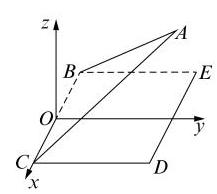
\includegraphics[width=0.2\textwidth]{bodyxb/src/117_1313_1747_217_194_0.jpg}
        \end{center}

        法二: 设 $F,G$ 分别为 ${BC},{DE}$ 的中点, 连接 ${AF},{FG}$ ,在正三角形 ${ABC}$ 中, ${AF} \bot  {BC},{AF} = \sqrt{3}$ ,在正方形 ${BCDE}$ 中, ${FG}//{CD},{FG} \bot  {BC},{FG} = {CD} = 2$ ,所以 $\angle {AFG}$ 为二面角 $A - {BC} - D$ 的平面角,即 $\angle {AFG} = \dfrac{\pi }{6},\vv{AC} \cdot  \vv{BD} = (\vv{AF} +  \vv{FC} \cdot  \left( {\vv{BC} + \vv{CD}}\right)  = \left( {\vv{AF} + \dfrac{1}{2}\vv{BC}}\right)  \cdot  \left( {\vv{BC} + \vv{FG}}\right)  = \vv{AF}$ . $\vv{BC} + \vv{AF} \cdot  \vv{FG} + \dfrac{1}{2}\vv{BC} + \dfrac{1}{2}\vv{BC} \cdot  \vv{FG} = \sqrt{3} \times  2 \times  \left( {-\cos \dfrac{\pi }{6}}\right)  + \dfrac{1}{2} \times  {2}^{2} =  - 1.$
        \begin{center}
        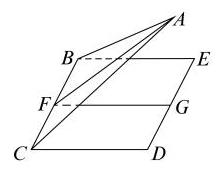
\includegraphics[width=0.2\textwidth]{bodyxb/src/117_1315_2006_216_169_0.jpg}
        \end{center}
    \end{jieda}

    \item (2025$\cdot$普陀区一模$\cdot$9)设 $\lambda  \in  \mathbf{R}$ ，在如图所示的平行六面体 ${ABCD} - {A}_{1}{B}_{1}{C}_{1}{D}_{1}$ 中， $\angle {A}_{1}{AB} =  \angle {A}_{1}{AD} = \angle {BAD} = \dfrac{\pi }{3},A{A}_{1} = 2,{AB} = {AD} = 1$ ,点 $M$ 是棱 ${C}_{1}{D}_{1}$ 的中点， $\vv{{A}_{1}N} = \lambda \vv{{A}_{1}{D}_{1}}$ ，若 $\vv{AM} \cdot  \vv{CN} = 2$ ,则 $\lambda$ 的值为\blkda[2]{$\dfrac{1}{3}$}.

    \begin{center}
    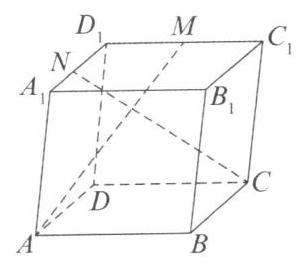
\includegraphics[width=0.2\textwidth]{bodyxb/src/159_1017_1734_298_264_0.jpg}
    \end{center}


    \begin{jieda}
        设 $\vv{AB} = \vv{a},\vv{AD} = \vv{b},\vv{A{A}_{1}} = \vv{c}$ , 由 $\angle {A}_{1}{AB} = \angle {A}_{1}{AD} = \angle {BAD} = \dfrac{\pi }{3}$ , $A{A}_{1} = 2,{AB} = {AD} = 1$ ,可得 $\left| \vv{a}\right|  = \left| \vv{b}\right|  = 1,\left| \vv{c}\right|  = 2,\vv{a} \cdot  \vv{b} = \dfrac{1}{2},\vv{a} \cdot  \vv{c} = \vv{b} \cdot  \vv{c}  = 1$ ,因为点 $M$ 是棱 ${C}_{1}{D}_{1}$ 的中点, $\vv{{A}_{1}N} = \lambda \vv{{A}_{1}{D}_{1}}$ ,所以 $\vv{AM}$ . $\vv{CN} = \left( {\vv{A{A}_{1}} + \vv{{A}_{1}{D}_{1}} + \vv{{D}_{1}M}}\right)  \cdot  \left( {\vv{AN} - \vv{AC}}\right)  = \left( {\vv{c} + \vv{b} + \dfrac{1}{2}\vv{a}}\right)$ . $\left\lbrack  {\vv{c} + \lambda \vv{b} - \left( {\vv{a} + \vv{b}}\right) }\right\rbrack   = \left( {\dfrac{1}{2}\vv{a} + \vv{b} + \vv{c}}\right)  \cdot  \left\lbrack  {-\vv{a} + \left( {\lambda  - 1}\right) \vv{b} + \vv{c}}\right\rbrack  =  - \dfrac{1}{2}{\vv{a}}^{2} + \left( {\lambda  - 1}\right) {\vv{b}}^{2} + {\vv{c}}^{2} + \dfrac{\lambda  - 3}{2}\vv{a} \cdot  \vv{b} - \dfrac{1}{2}\vv{a} \cdot  \vv{c} + \lambda \vv{b} \cdot  \vv{c} =  - \dfrac{1}{2} + \lambda  - 1 + 4 + \dfrac{\lambda  - 3}{4} - \dfrac{1}{2} + \lambda  = \dfrac{9\lambda }{4} + \dfrac{5}{4} = 2$ ,解得 $\lambda  = \dfrac{1}{3}$.
        \begin{center}
            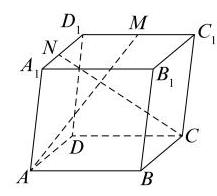
\includegraphics[width=0.2\textwidth]{bodyxb/src/118_647_540_217_196_0.jpg}
        \end{center}
    \end{jieda}

    \item (2024$\cdot$静安区一模$\cdot$9)如图所示，在四棱锥 $P - {ABCD}$ 中， ${PA}\bot$ 平面 ${ABCD}$ ，底面 ${ABCD}$ 是矩形， $\left| {AP}\right|  = \left| {AB}\right|  = 2,\left| {AD}\right|  = 4,E$ 是 ${BC}$ 上的点， 直线 ${PB}$ 与平面 ${PDE}$ 所成的角是 $\arcsin \dfrac{\sqrt{3}}{6}$ ，则 ${BE}$ 的长为\blkda[2]{2}.

    \begin{center}
    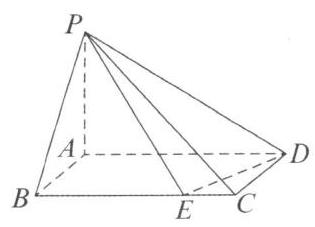
\includegraphics[width=0.2\textwidth]{bodyxb/src/160_1182_172_315_227_0.jpg}
    \end{center}
    \begin{jieda}
        由题意知在四棱锥中, ${PA} \bot$ 平面 ${ABCD}$ ,底面 ${ABCD}$ 是矩形，以 $A$ 为坐标原点，以射线 ${AB},{AD},{AP}$ 为 $x,y,z$ 轴的正半轴建立空间直角坐标系,则 $A(0$ , $0,0),B\left( {2,0,0}\right) ,P\left( {0,0,2}\right) ,D(0$ , $4,0)$ ,设 $E\left( {2,t,0}\right) \left( {0 \leq  t \leq  4}\right)$ ,则 $\vv{PB} = \left( {2,0, - 2}\right) ,\vv{PD} = (0$ , $4, - 2),\vv{PE} = \left( {2,t, - 2}\right)$ ,设平面 ${PDE}$ 的一个法向量为 $\vv{n} =  \left( {x,y,z}\right)$ ,则 $\left\{  \begin{array}{l} \vv{n} \cdot  \vv{PD} = 0 \\  \vv{n} \cdot  \vv{PE} = 0 \end{array}\right.$ ,即 $\left\{  \begin{array}{l} {4y} - {2z} = 0 \\  {2x} + {ty} - {2z} = 0 \end{array}\right.$ ,令 $y = 2$ ,则 $\vv{n} = \left( {4 - t,2,4}\right)$ ,设直线 ${PB}$ 与平面 ${PDE}$ 所成的角为 $\theta ,\theta  \in  \left\lbrack  {0,\dfrac{\pi }{2}}\right\rbrack$ ,直线 ${PB}$ 与平面 ${PDE}$ 所成的角是 $\arcsin \dfrac{\sqrt{3}}{6}$ ,则 $\sin \theta  = \dfrac{\sqrt{3}}{6}$ ,故 $\sin \theta  = \left| {\cos \langle \vv{n},\vv{PB}\rangle }\right|  = \dfrac{\left| \vv{n} \cdot  \vv{PB}\right| }{\left| \vv{n}\right| \left| \vv{PB}\right| } =  \dfrac{\left| 2t\right| }{2\sqrt{2} \cdot  \sqrt{{\left( 4 - t\right) }^{2} + {20}}} = \dfrac{\sqrt{3}}{6}$ ,解得 $t = 2$ ,故 ${BE} = 2$ .

        \begin{center}
        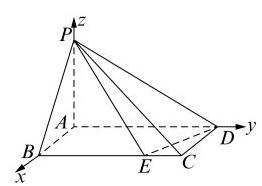
\includegraphics[width=0.2\textwidth]{bodyxb/src/118_607_1193_262_186_0.jpg}
        \end{center}
    \end{jieda}

    \item (2025$\cdot$黄浦区一模$\cdot$8)在正四面体 ${ABCD}$ 中，点 $N$ 是 $\bigtriangleup  {ABC}$ 的中心，若 $\vv{DN} = \lambda \vv{DA} + \mu \vv{DB} +  \nu \vv{BC}\left( {\lambda ,\mu ,\nu  \in  \mathbf{R}}\right)$ ，则 $\lambda  + \mu  + \nu  =$ \blkda[2]{$\dfrac{4}{3}$}.
    \begin{jieda}
        $\vv{DN} = \lambda \vv{DA} + \mu \vv{DB} +  \nu (\vv{DC} - \vv{DB}) = \lambda \vv{DA} + (\mu - \nu) \vv{DB} + \nu \vv{DC} = \dfrac{1}{3} \vv{DA} + \dfrac{1}{3} \vv{DB} + \dfrac{1}{3} \vv{DC}$

        故$\left\{\begin{array}{l}
            \lambda = \dfrac{1}{3} \\
            \mu = \dfrac{2}{3} \\
            \nu = \dfrac{1}{3}
        \end{array}\right.$
    \end{jieda}
\end{enumerate}

\subsection*{排列组合}
\begin{enumerate}
    \item (2024$\cdot$闵行区二模$\cdot$7)现有 5 个工程队承建某工程的 5 个不同项目，每个工程队承建一个项目， 其中甲工程队不能承建 $A$ 项目,则不同的承建方案有\blkda[2]{96}种. (用数字作答)
    \item (2025$\cdot$宝山区一模$\cdot$7)已知关于正整数 $x$ 的方程 ${{C}}_{12}^{x - 1} = {{C}}_{12}^{{5x} - 5}$ ，则该方程的解为\blkda[2]{1或3}.
    \item (2025$\cdot$闵行区一模$\cdot$8)从 10 名数学老师中选出 3 人安排在 3 天的假期中值班，每天有且只有一人值班. 若老师甲必须参加且不安排在假期第一天值班, 则不同的值班安排方法种数为\blkda[2]{144}.
    \item (2024$\cdot$徐汇区一模$\cdot$8)要排出高一某班一天上午 5 节课的课表，其中语文、数学、英语、艺术、体育各一节，若要求语文、数学选一门第一节课上，且艺术、体育不相邻上课，则不同的排法种数是\blkda[2]{24}.
    \item (2024$\cdot$闵行区一模$\cdot$9)今年中秋和国庆共有连续 8 天小长假，某单位安排甲、乙、丙三名员工值班，每天都需要有人值班. 任选两名员工各值 3 天班，剩下的一名员工值 2 天班，且每名员工值班的日期都是连续的，则不同的安排方法数为\blkda[2]{18}.
    \item (2025$\cdot$上海秋季卷$\cdot$9)4 个家长和 2 个儿童去爬山，6 个人需要排成一条队列，要求队列的头和尾均是家长，则不同的排列个数有\blkda[2]{288}种.
    \item (2025$\cdot$虹口区二模$\cdot$10)已知 9 个小球的编号为 1、2、...、9，从中有放回地摸取小球三次，并依次记录其编号，若这三个编号成等差数列，则共有\blkda[2]{41}种不同的摸取方法.
    \begin{jieda}
        若三个编号成等差数列, 若三个编号相同, 共有 9 种,若三个编号彼此都不相同,设这三个编号为 $a,b,c$ ,则 ${2b} = a + c$ ,则 $a,c$ 同为奇数或同为偶数,则 $b$ 可由 ${2b} = a + c$ 来确定, 奇数编号的小球共 5 个, 偶数编号的小球共 4 个, 若 $a,c$ 同为奇数，则 $a,c$ 的选择方法种数为 $2{{C}}_{5}^{2} = {20}$ 种；若 $a$ 、 $c$ 同为偶数,则 $a,c$ 的选择方法种数为 $2{{C}}_{4}^{2} = {12}$ 种. 当三个编号彼此不同时,不同的摸法种数为 ${20} + {12} = {32}$ 种. 综上所述,不同的摸法种数为 $9 + {32} = {41}$ 种.
    \end{jieda}
    \item (2024$\cdot$上海秋季卷$\cdot$10)设集合 $A$ 中的元素皆为无重复数字的三位正整数，且元素中任意两者之积皆为偶数，求集合中元素个数的最大值\blkda[2]{329}.

    \begin{center}
    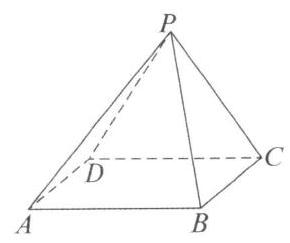
\includegraphics[width=0.2\textwidth]{bodyxb/src/211_1135_463_290_243_0.jpg}
    \end{center}
    \begin{jieda}
        由题意知集合中且至多只有一个奇数, 其余均是偶数. 首先讨论三位数中的偶数,  \ding{172}  当个位为 0 时, 则百位和十位在剩余的 9 个数字中选择两个进行排列, 则这样的偶数有 ${{P}}_{9}^{2} = {72}$ 个； \ding{173}  当个位不为 0 时，则个位有 ${{C}}_{4}^{1}$ 个数字可选， 百位有 ${{C}}_{8}^{1}$ 个数字可选，十位有 ${{C}}_{8}^{1}$ 个数字可选，根据分步计数原理这样的偶数共有 ${{C}}_{4}^{1}{{C}}_{8}^{1}{{C}}_{8}^{1} = {256}$ ; 然后再加上一个三位正奇数，得集合中元素个数的最大值为 ${72} + {256} + 1 = {329}$ 个.
    \end{jieda}
    \item (2024$\cdot$杨浦区二模$\cdot$10)有 5 名志愿者报名参加周六、周日的公益活动，若每天从这 5 人中安排 2 人参加，则恰有 1 人在这两天都参加的不同安排方式共有\blkda[2]{60}种.
    \begin{jieda}
        $N = {{C}}_{5}^{1}{{C}}_{4}^{1}{{C}}_{3}^{1} = {60}$ .
    \end{jieda}
    \item (2024$\cdot$徐汇区二模$\cdot$10)如图所示，将一个四棱锥的每一个顶点染一种颜色，并使同一条棱上的两端点异色，如果只有 4 种颜色可供使用，则不同的染色方法有\blkda[2]{72}种.
    \begin{jieda}
        下面分两种情况,即 $C,A$ 同色与 $C,A$ 不同色来讨论. (1) $P$ 的着色方法有 4 种, $A$ 的着色方法有 3 种, $B$ 的着色方法有 2 种, $C,A$ 同色时, $C$ 的着色方法为 1 种, $D$ 的着色方法有 2 种. ( 2 ) $P$ 的着色方法有 4 种， $A$ 的着色方法有 3 种， $B$ 的着色方法有 2 种. $C$ 与 $A$ 不同色时 $C$ 的着色方法有 1 种, $D$ 的着色方法有 1 种,综上,两类共有 $4 \times  3 \times  2 \times  1 \times  2 + 4 \times  3 \times  2 \times  1 \times  1 = {48} + {24} = {72}$ (种).
    \end{jieda}
\end{enumerate}
\subsection*{二项式定理}
\begin{enumerate}
    \item (2024$\cdot$崇明区二模$\cdot$7)若$(x+a)^{5}$ 的二项式展开式中 ${x}^{2}$ 的系数为 10，则 $a =$ \blkda[2]{1}.

    \item (2025$\cdot$浦东新区二模$\cdot$7)在$\left(x - \dfrac{1}{x}\right)^{10}$ 的二项展开式中，常数项为\blkda[2]{$-252$}.

    \item (2025$\cdot$松江区一模$\cdot$7)已知 ${\left( x + 2\right) }^{4} = {a}_{0} + {a}_{1}x + {a}_{2}{x}^{2} + {a}_{3}{x}^{3} + {a}_{4}{x}^{4}$ ，则 ${a}_{1} + {a}_{2} + {a}_{3} + {a}_{4} =$ \blkda[2]{$65$}.

    \item (2024$\cdot$嘉定区一模$\cdot$8)在$(1+2x)^{6}$ 的二项展开式中，系数最大的项为\blkda[2]{${240}{x}^{4}$}.

    \item (2024$\cdot$宝山区一模$\cdot$8)若对于任意实数 $x$ ，都有 ${x}^{4} = {a}_{0} + {a}_{1}\left( {x + 2}\right)  + {a}_{2}{\left( x + 2\right) }^{2} + {a}_{3}{\left( x + 2\right) }^{3} +  {a}_{4}{\left( x + 2\right) }^{4}$ ，则 ${a}_{3}$ 的值为\blkda[2]{$-8$}.

    \item (2023$\cdot$上海春季卷$\cdot$8)设$(1-2x)^4 = {a}_{0} + {a}_{1}x + {a}_{2}{x}^{2} + {a}_{3}{x}^{3} + {a}_{4}{x}^{4}$ ，则 ${a}_{0} + {a}_{4} =$ \blkda[2]{17}.

    \item (2025$\cdot$青浦区一模$\cdot$9)$(x + y)(x - y)^{6}$ 的展开式中， ${x}^{4}{y}^{3}$ 项的系数为\blkda[2]{$-5$}.
    \begin{jieda}
        ${\left( x - y\right) }^{6}$ 展开式的通项为 ${T}_{r + 1} = {{C}}_{6}^{r}{x}^{6 - r}{\left( -y\right) }^{r},r \in  \{ 0,1,2,3,4,5,6\}$ ,所以含 ${x}^{4}{y}^{3}$ 的项为 $x{{C}}_{6}^{3}{x}^{3}{\left( -y\right) }^{3} + y{{C}}_{6}^{2}{x}^{4}  {\left( -y\right) }^{2} =  - 5{x}^{4}{y}^{3}$ ,即 ${x}^{4}{y}^{3}$ 项的系数为 -5 .
    \end{jieda}

    \item (2023$\cdot$上海秋季卷$\cdot$10)已知$(1+2023x)^{100} + {\left( {2023} - x\right) }^{100} = {a}_{0} + {a}_{1}x + {a}_{2}{x}^{2} + \cdots  + {a}_{100}{x}^{100}$ ，且 $k \in  \{ 0,1,2,3,\cdots ,{100}\}$ ，当 ${a}_{k} < 0$ 时，正整数 $k$ 的最大值为\blkda[2]{$49$}.
    \begin{jieda}
        ${a}_{k} = {{C}}_{100}^{k}{2023}^{k} + {\left( -1\right) }^{k}{{C}}_{100}^{k}{2023}^{{100} - k} < 0$ ,依题意 $k$ 为奇数，所以 ${2023}^{k} < {2023}^{{100} - k},k < {100} - k \Longrightarrow  k < {50} \Longrightarrow  {k}_{\max } = {49}$ .
    \end{jieda}

    \item (2024$\cdot$金山区一模$\cdot$10)若$(10x + 6y)^{3} = a{x}^{3} + b{x}^{2}y + {cx}{y}^{2} + d{y}^{3}$ ，则 $- a + {2b} - {4c} + {8d} =$ \blkda[2]{$8$}.
    \begin{jieda}
        令 $x =  - 1,y = 2$ ,则 ${\left( {10} \times  \left( -1\right)  + 6 \times  2\right) }^{3} =  - a + {2b} - {4c} + {8d}$ ,所以 $- a + {2b} - {4c} + {8d} = {2}^{3} = 8$
    \end{jieda}
\end{enumerate}